%!TEX root=report.tex
\subsection{Kernel Principal Component Analysis (Kernel PCA)}

Before delving into kernel methods, the standard PCA method will briefly be recapped.
 PCA as introduced in this report was done via SVD ($X=U\Sigma V^T$); the columns of $U$ were the eigenvectors of $XX^T$ and the columns of $Z$ where $Z=U\Sigma$ constituted a basis in the PCA-vectorspace ($Z$); these columns were referred to as the principal components (PCs). 
Looking at the dependencies of $U$ it is apparent that the PCs will end up being linear combinations of basis in original input space $X$. 
In most cases this suffices but what if there are no linear relationships in the $X$ space, standard PCA won't be appropriate.
Below is a concrete example

\begin{figure}[H]
	\center
	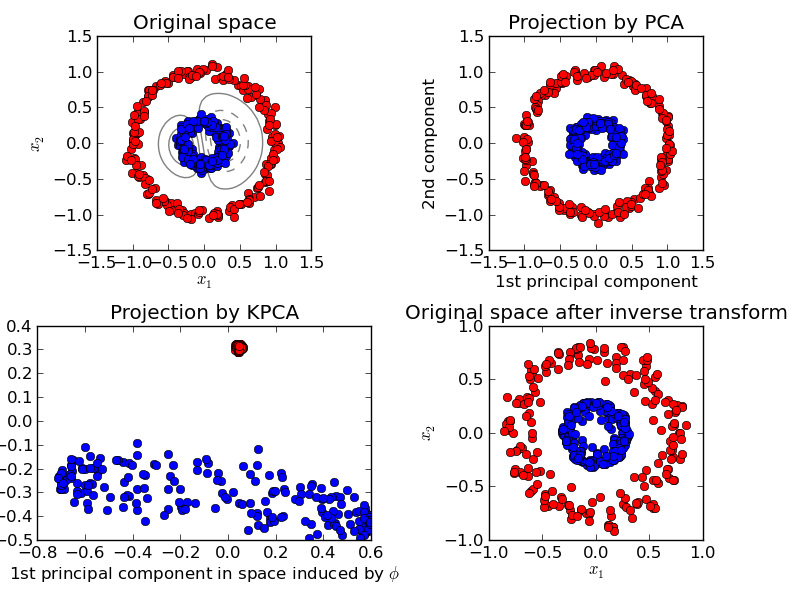
\includegraphics[width=\textwidth]{figures/kernel_pca_example.png}
	\caption{Motivating kernel PCA example. Image courtesy of scikit-learn. http://scikitlearn.org/stable/auto\_examples/decomposition/plot\_kernel\_pca.html }
	\label{fig:motivation_kernelpca}
\end{figure}.
As is seen in the figure above, classes that wasn't linearly separable in the Original space can be become linearly separable in the kernel space. This in turn makes clustering much easier and hopefully improves results.

\subsubsection{The Kernel Trick}

The following two sections are heavily influenced by a video lecture from youtube \cite[from minutes 10-30]{youtube-caltech}. In kernel PCA, instead of working on the inner product $(X,X^T)$ we are interested in using a nonlinear mapping $\Phi: X\rightarrow Y$, such that the singular value decomposition is carried out on $(\Phi(X),\Phi(X^T))=(Y,Y^T)=K(X,X^T)$; this inner product in the $Y$-space is called the kernel. 
So for something to be a valid kernel, all it needs to satisfy is for the kernel to a function of an inner production in some vector space.
For the above to become more clear, let us give an example of a polynomial kernel in a 2-dimensional $X$-space. in the following $X$ is a vector and $X'$ is simply some other vector in the same space as $X$:

\begin{equation}
K(X,X')=(1+X^T X')^2=(1+x_1^T x_1^{'}+x_2^T x_2 ')^2=1+x_1^2 {x_1 '}^2 +2 x_1 x_1 '+2 x_2 x_2 '+2 x_1 x_1 ' x_2 x_2'
\end{equation}

So for the above to actually be a true kernel there would have to be some vector space $Y$ in which the above was an inner product. From the coefficients above it can be deduced that the basis in the $Y$ must be given as
\begin{equation}
(1,x_1^2,x_2^2,\sqrt{2} x_1, \sqrt{2} x_2 , \sqrt{2} x_1 x_2)
\end{equation}
So why is the above important. Imagine if one were to increase the power from 2 to i.e. 100: $K(X,X')=(1+X^T X')^100$. Calculating the kernel in the $X$-space is easy; $(1+X^T X')$ is just a number and raising it to the power of 100 can be done quickly. 
On the other hand if one were to explicitly calculate the kernel as the inner product in the the $Y$-space, you would first have to compute a more than 100-d vector, transpose it, multiply the terms and sum them - i.e. not very efficient and imagine if $X$ had a dimension of 100 instead of 2 - you would end up with too many variables for the computation to be possible.

 All of the above is denoted as the Kernel Trick. It simples is the process of utilizing the fact that the inner product in the $Y$-space can be carried out without knowing the explicit mapping $\Phi$ and as we will show in the next section $\Phi$ can even be a mapping to an infinite dimensional space in which case it would be impossible to actually carry out this transformation.

\subsubsection{The Radial Basis Function (RBF) kernel}
Due to the trigonometric nature of the GRACE data ( remember the fourier expansion with sines and cosines) the appropriate kernel has been deemed to be RBF. The RBF kernel is defined as
\begin{equation}
K(X,X')=exp(-\gamma ||X-X'||^p)
\end{equation}
Now the above can easily be calculated, but one needs to be sure that it actually corresponds to a straight inner product in some vector space $Y$. 
For simplification, in the following proof $\gamma=1$, $p=2$ and $X$ is one dimensional (a scalar).
\pagebreak
\begin{subequations}
Proof: $\exists \Phi \rightarrow K(X,X')=exp(- ||X-X'||^2)=K(\Phi(X),\Phi(X'))$\\
\begin{align}
K(x,x')=exp(- ||x-x'||^2)=exp(- (x-x')^2)  \\
=exp(-x^2) exp(-{x'}^2) exp(2 x x') \\
\text{since } exp(2 x x') \text{ can be Taylor expanded to} \sum_{k=0}^\infty \frac{2^k(x)^k (x')^k}{k!} \text{ it follows that:}  \\
 =\sum_{k=0}^\infty [(\sqrt{\frac{2^k}{k!}} (x)^k exp(-x^2))(\sqrt{\frac{2^k}{k!}} (x')^k exp(-{x'}^2))  ]
\end{align}
\end{subequations}
From the above it is seen that for any k the term in the right parenthesis is exactly equal to the left paranthesis if $x'$ was substituted with $x$ - thus it is an inner product. Since the sum is infinite it is the inner product in a infinite dimensional space.
 So one can know trust that RBF actually is a valid kernel.

\subsubsection{Final notes of kernel PCA}
Remember that in the SVD the columns of $U$ was the eigenvectors of $K(X,X^T)$ and the columns of $V$ the eigenvectors of $K(X^T,X)$. The size of those is going to be NxN and DxD respectively where N is the number of samples and D the dimensions in X. 
So in the case of clustering with positions on rows and days on columns in $X$, the shape is 64800x341. 
The resulting amount of ram required to hold an 64800x64800 matrix of float32 numbers is $64800*64800*32/8/1024/1024/1024=15.64 gb$. Now on this ram block the chosen SVD library needs to factorize into $U\Sigma V$ so one probably needs quite a bit more ram. So to carry out Kernel PCA on datasets of sizes larger than 10000 samples we recommend some form of cloud computing (or a really expensive stationary pc.)